\documentclass[11pt,oneside,bibtotoc,liststotoc]{scrbook}


\usepackage{graphicx}
\usepackage[ngerman]{babel}
\usepackage[utf8]{inputenc}
\usepackage{a4wide}
\usepackage{parskip}
\usepackage[bookmarks]{hyperref}
\usepackage[right]{eurosym}
\usepackage{amsmath}
\usepackage{siunitx}
\sisetup{locale = DE} 

\usepackage{float}

\usepackage[hang,nooneline,bf]{caption}
\usepackage{booktabs}
\usepackage{dcolumn}                  % Ausrichtung nach Dezimalpunkt in Tabellen
\newcolumntype{.}{D{.}{.}{-1}}
%\usepackage{setspace}
\pagestyle{headings}
%\setlength{\textwidth}{15cm}
%\setlength{\textheight}{22.5cm}
%\setlength{\oddsidemargin}{1cm}
%\setlength{\evensidemargin}{0cm}
% \renewcommand{\baselinestretch}{1.2}
% \parskip1ex plus0.5ex minus0.5ex
\usepackage[onehalfspacing]{setspace}  % setzt den Zeilenabstand auf 1,5 fach
\usepackage{multirow}

% Zur Einbindung von Excel
\usepackage{xcolor}
\usepackage{colortbl}
\usepackage{rotating}
 
 %%%%% für Matlab
\usepackage{listings}
 
 %%%%%% für SVG Dateien
\usepackage{svg}
 
 %%%%% Roman numbers
\newcommand{\RomanNumeralCaps}[1]
{\MakeUppercase{\romannumeral #1}}     % Einbinden der Header Datei



\begin{document}
\thispagestyle{empty}
\graphicspath{{images/}}
\kern-13.5mm
\includegraphics[width=55mm]{image/Titel/logo_umit.pdf}
 


\vspace*{2cm}\par
\begin{center}

{\huge \textbf{ Laborpraktikum}} \\[1em]
%{\huge \textbf{Testautomat}}
\vspace{2cm}\par

{\large Prozessmesstechnik}
\vspace{1cm}\par
{\large LV-Nummer: 844192}
\vspace{1cm}\par
Lehrveranstaltungsleiter: Prof. Dr. Alexander Sutor \\
Semester: WS 22/23



von \\[1ex]
xxx xxxx \\
Stefan Kaufmann    51867606 
\vspace{1cm}\par

Innsbruck, Januar 2023

\end{center}

%------------- Ende Titelseite --------------------------------


\thispagestyle{empty}

\setcounter{page}{1}
\pagenumbering{Roman}
\renewcommand{\baselinestretch}{1.00}\normalsize
\tableofcontents
\listoffigures
\listoftables
\renewcommand{\baselinestretch}{1.5}\normalsize
\newpage
\setcounter{page}{1}
\pagenumbering{arabic}

%%%%%%%%%%%%%%%%%%%%%%%%%%%%%%%%%%%%%%   Einbinden der Kapitel %%%%%%%%%%%%%
\chapter{Einleitung} \label{Einleitung}

%Kurze Erläuterung der Aufgabenstellung und der Messmethode, d.h. stichwortartige 
%Zusammenstellung von wesentlichen Definitionen, Formeln, etc. (keine Herleitungen, 
%keine seitenlange Darstellung von Lehrbuchwissen!).  
\newpage
%input{content/2_Aufbau}
\newpage
%\chapter{Messungen} \label{Messungen}

Das nachfolgende Kapitel legt die Ergebnisse der Messungen dar. 



\section{Charakteisierung des Wandlers}

Die Ermittlung des Impedanzganges ist in \autoref{img:Impedanzgang} dargestellt. Hierbei wurde ein Serienwiederstand von \SI{51}{\Omega} verwendet. Der Impedanzgang weißt starke Ähnlichkeiten zum Impedanzgang eines Kondensators auf welche mit \(|Z| = \frac{1}{f c} \) Charakteisiert ist.


\begin{figure}[h]
    \centering
    \includesvg[width=1 \textwidth]{Berechnungen/Impedanzgang.svg}
    \caption{Impedanzgang des Piezowandlers}
    \label{img:Impedanzgang}
\end{figure}


Die genaue Untersuchung der Impedanz unterhalb der ersten Resonanz ist in \autoref{img:Impedanzgang_unten} dargestellt. Hierbei wird der Impedanzgang mit \SI{51}{\Omega} und \SI{2200}{\Omega} gegenübergestellt.

\begin{figure}[h]
    \centering
    \includesvg[width=1 \textwidth]{Berechnungen/Impedanzgang_unten.svg}
    \caption{Impedanzgang unterhalb der ersten Resonanz}
    \label{img:Impedanzgang_unten}
\end{figure}




\section{Messung der Schallgeschwindigkeit} \label{Aufbau_Schall}
Zur Messung der Schallgeschwindigkeit wird im ersten Versuchsaufbau ein Probenkörper mit der Breite \SI{30}{mm} verwendet. Die Dicke des Piezos beträgt  \SI{2}{mm}. Es ergibt sich eine Laufzeit von \SI{6.1e-6}{s}. Beim zweiten Versuch eribt die Laufzeit \SI{10.3e-6}{s}.
Über den Zusammenhang  \(c=\frac{\lambda}{T}\) ergeben sich die Ausbreitungsgeschwindigkeiten zu :

\begin{equation*}
    \begin{split}
    c = \frac{\lambda}{T} = \frac{32 mm}{6.1e-6 s} = 5245.90 \frac{m}{s}  \\[.4cm]
    c = \frac{62 mm}{6.1e-6 s} = 6019.41 \frac{m}{s}  
    \end{split}
\end{equation*}




\section{Materialprüfung}

Die nachfolgende Tabelle stellt die Ergebnisse der Laufzeit der einzelnen Probekörpern bei unterschiedlichen Frequnezen dar. Alle Messungen befinden sich dabei  zwischen  \SI{5.58}{\micro s} und  \SI{6.10}{\micro s}.


\begin{table}[H]
    \centering
    \begin{tabular}{l|llll}
         Probekörper Nr. &  \SI{800}{kHz} & \SI{1}{MHz} & \SI{1.4}{MHz} &  \\
         \hline
         1 & 5.58  & 6.10 & 5.38 &   \\
         2 & 5.30  & 5.50 & 5.42 &  \\
         3 & 5.52  & 5.46 & 5.38 &  
    \end{tabular}
    \caption{Laufzeitmessung bei unterschiedlichen Frequnezen und Empfangsamplitude}
    \label{tab:Materialprüfung}
\end{table}


\autoref{img:Materialprufung} stellt die Laufzeitmessungen der Probekörper bei \SI{1}{MHz} gegenüber. Dabei weisen die Amplitudenantworten abhängig vom untersuchten Körper unterschiedliche Amplituden auf. Die Schwingungsantwort von Probekörper eine weißt dabei die geringste und jene vom Körper 3 die größte Amplitde auf.


\begin{figure}
    \begin{minipage}[b]{.50\linewidth} % [b] => Ausrichtung an \caption
       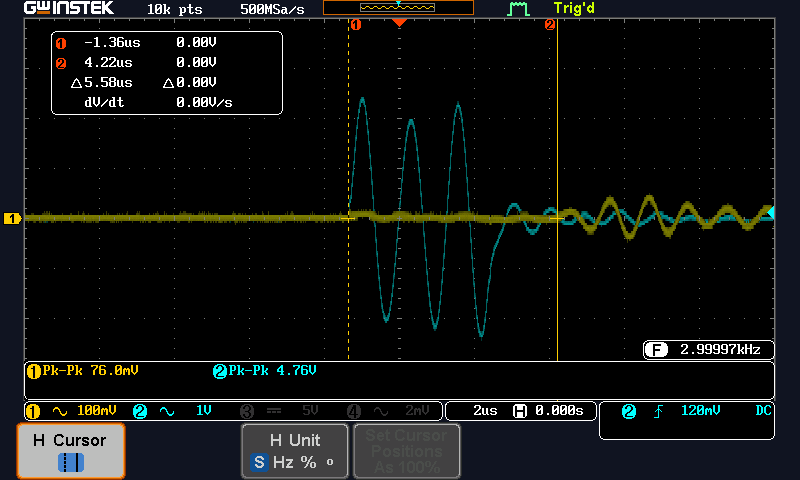
\includegraphics[width=\linewidth]{image/1_Quer.PNG}
       \caption*{\textbf{a)} Probekörper 1}
    \end{minipage}
    \hspace{.01\linewidth}% Abstand zwischen Bilder
    \begin{minipage}[b]{.5\linewidth} % [b] => Ausrichtung an \caption
       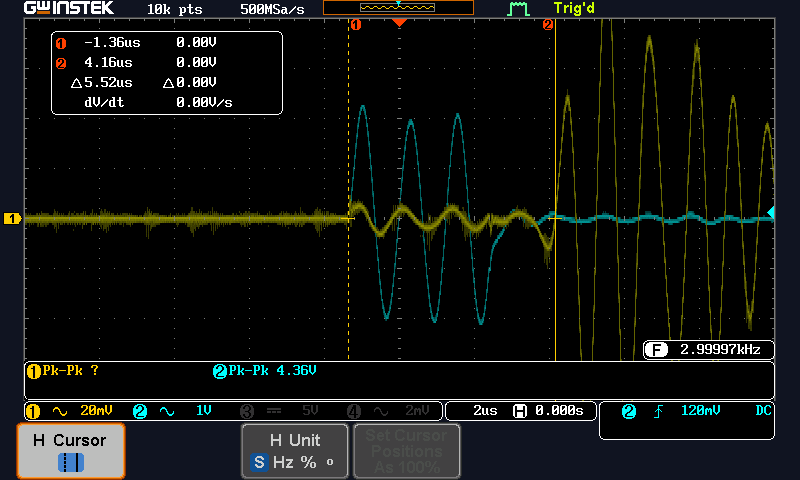
\includegraphics[width=\linewidth]{image/2_quer.PNG}
       \caption*{\textbf{b)} Probekörper 2}
    \end{minipage}

    \begin{minipage}[b]{.50\linewidth} % [b] => Ausrichtung an \caption
        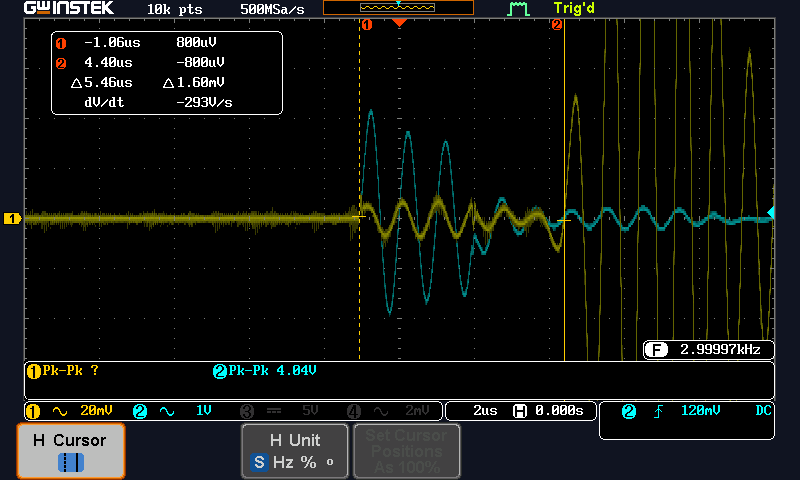
\includegraphics[width=\linewidth]{image/3_quer.PNG}
        \caption*{\textbf{a)} Probekörper 3}
     \end{minipage}
     \hspace{.01\linewidth}% Abstand zwischen Bilder
     
    \caption{Gegenüberstellung der Laufzeitmessung bei einer Anregung von \(V_{pp}= \SI{5}{V}, f= \SI{1}{MHz}\)}
    \label{img:Materialprufung}
 \end{figure}
\newpage
%\chapter{Einleitung} \label{Einleitung}

%Kurze Erläuterung der Aufgabenstellung und der Messmethode, d.h. stichwortartige 
%Zusammenstellung von wesentlichen Definitionen, Formeln, etc. (keine Herleitungen, 
%keine seitenlange Darstellung von Lehrbuchwissen!). 
\newpage
%\chapter{Einleitung} \label{Einleitung}

%Kurze Erläuterung der Aufgabenstellung und der Messmethode, d.h. stichwortartige 
%Zusammenstellung von wesentlichen Definitionen, Formeln, etc. (keine Herleitungen, 
%keine seitenlange Darstellung von Lehrbuchwissen!). 







% Das Literaturverzeichnis

\bibliographystyle{IEEEtran}
%\bibliography{Literatur}
\clearpage

%\input{4_Anhang}


\end{document}
